%
%  Thesis Vorlage für die Hochschule Heilbronn
%
%  Created by Prof. Dr. Detlef Stern on 2010-08-14.
%  Updated by Valentin Weber on 2020-10-05.
%  Copyright (c) 2020 . All rights reserved.
%
\documentclass[12pt,toc=bib,toc=listof]{scrreprt}
\usepackage[ngerman]{babel} 
\usepackage[utf8]{inputenc}
\usepackage[T1]{fontenc}
\usepackage{lmodern}
\usepackage{setspace}
\usepackage{geometry}

\usepackage{hyperref}
\hypersetup{
  ,colorlinks=true
  ,linkcolor=blue
  ,citecolor=blue
  ,filecolor=blue
  ,urlcolor=blue
  }

% Fachbezogene Werte (müssen aktualisiert werden)
\newcommand{\hhnsubject}{COMPUTER AND ROBOTVISION}
\newcommand{\hhnsubjectnum}{PRÜFUNGSNUMMER: 135031}
\newcommand{\hhnlecturer}{PROF. DR. DIETER MAIER}

% Vom Studierenden zu aendernde Werte
\newcommand{\reprttopic}{BRIEFMARKENERKENNUNG}
\newcommand{\reprtstudentname}{GEORG JAHN, MARTIN HAAG}
\newcommand{\reprtstudentid}{195XXX, 194980}
\urldef{\reprtstudentmail}\url{gjahn@stud.hs-heilbronn.de ,mahaag@stud.hs-heilbronn.de}

\usepackage{ifpdf}
\ifpdf
\usepackage[pdftex]{graphicx}
\else
\usepackage{graphicx}
\fi

\usepackage[headsepline]{scrlayer-scrpage}
\pagestyle{scrheadings}
\clearscrheadfoot
\ihead{\hhnsubject: \reprttopic}
\ohead{\pagemark}
\renewcommand*{\chapterpagestyle}{scrheadings}
\renewcommand*{\chapterheadstartvskip}{}

%meine adds
\usepackage[belowskip=-15pt,aboveskip=0pt]{caption}
\renewcaptionname{ngerman}\figurename{Abb.}	
\usepackage{caption}
\captionsetup{format=plain}

% Deckblatt Definitionen (begin)
\titlehead{\flushright
\includegraphics{./bilder/hhn.png}}
\subject{{\hhnsubject{} (\hhnsubjectnum{})}}
\title{\reprttopic}
\author{\reprtstudentname\footnote{\reprtstudentid, \reprtstudentmail}}
%% Datum nie auf einen festen Wert setzen
\publishers{Eingereicht bei \hhnlecturer}
% Deckblatt Definitionen (end)

\begin{document}
\renewcommand*{\figurename}{Abb.}
\pagenumbering{Roman} 
\selectlanguage{ngerman}
\maketitle
\newgeometry{left=30mm, top=25mm, right=15mm, bottom=25mm}

\tableofcontents

\addchap{List of Abbreviations} % (fold)
\label{sec:listofabbrv}

\addchap{Abkürzungsverzeichnis} % (fold)
\label{sec:abkuerzungsverzeichnis}

\begin{description}
  \item[ABK:] ABKÜRZUNG 
\end{description}

% chapter abkuerzungsverzeichnis (end)

\onehalfspacing

\addchap{Management Summary} % (fold)
\label{cha:management_summary}
\ldots

% chapter management_summary (end)
\newpage
\pagenumbering{arabic}

% report (begin)
\chapter{Einleitung} % (fold)
\label{sec:einleitung}

\section{Motivation} % (fold)
\label{sec:motivation}

Bildverarbeitung ist kein neues Feld der Forschung mehr und auch neuronale Netzwerke sind bereits seit vielen Jahren Subjekt von ständiger Weiterentwicklung. Da diese beiden Fachgebiete durchaus gut miteinander harmonieren haben wir uns entschieden, in unserem Projekt eine Aufgabe die beides benötigt zu bearbeiten. Im Rahmen useres CRV Projektes haben wir deshalb die Unterscheidung von Briefmarken in gestempelte und ungestempelte automatisiert, durchgeführt. Wenn auch unsere Arbeit sehr unwahrscheinlich kommerzielle Anwendung findet, ist es doch geeignet um an einem Tag der offenen Tür oder einem "studieren probieren" Event demonstriert zu werden.

% section motivation (end)

\section{Ziel der Arbeit} % (fold)
\label{sec:ziel_der_arbeit}
Das Ziel der Arbeit war es, mit Hilfe eines Teils "klassischer" Bildverarbeitung und eins neuronalen Netzwerkes Bilder von gestempelten von Bildern mit ungestempelten Briefmarken zu unterscheiden.
Ursprünglich war der Plan mit Bildern von ganzen Briefen zu arbeiten. Der Vorteil bei diesem Ansatz wäre, dass die Überlappung des Stempels über Briefmarke und Brief es wohl für das Netzwerk einfacher gemacht hätte die Klassen gestempelt/nicht gestempelt zu unterscheiden. Auf Grund von Datenschutzgesetzten waren wir jedoch nicht in der Lage, einen ausreichend großen Datensatz zusammen zu tragen. Deshalb haben wir uns entschieden, eine alte selbst gesammelte Briefmarkensammlung abzufotografieren und somit zu digitalisieren.


Dieser selbst generierte Datensatz ist zwar auch nicht groß genug um ein ernsthaftes Training mit einem NN durchzuführen, reicht aber für einen "Proof of concept"

% section ziel_der_arbeit (end)

\section{Vorgehensweise} % (fold)
\label{sec:vorgehensweise}

Unser Vorgehen teilt sich in zwei Teilschritte auf:
\begin{itemize}
\item "klassische" Bildverarbeitung:\\ 
Dabei werden die Bilder so vorverarbeitet, dass sie als Input für das NN dienen können. Das wird mit Hilfe von helligkeitsbasierte Binarisierung und einigen morphologischen Filtern erreicht. Außerdem kommen noch Schritte zum drehen des Bildes zum Einsatz. Das Endergebniss dieser Bildverarbeitungsschritte ist ein rechteckiger Bildausschnitt, der nur die Briefmarke enthält. 

\item Klassifizierung mit einem NN:\\
In diesem Bereich der Arbeit wird der vorverarbeitete Datensatz für das Training und die Evaluierung des NN aufbereitet. Außerdem wird das NN selbst hier erstellt. Da wir die Technik des Transferlearning genutzt haben, wurde hier nur ein vortrainiertes Model herausgesucht und das Outputlayer ausgetauscht.

\end{itemize}

% section vorgehensweise (end)
% chapter einleitung (end)

\chapter{Klassische Bildverarbeitung} % (fold)
\label{sec:klass_bv}

\section{Übersicht}
\label{sec_bv:übersicht}
Das folgende Schaubild zeigt, welche Schritte vorgenommen werden und in welcher Reihenfolge. Dafür wurde ein Beispiel gewählt, bei dem keine Komplikationen auftreten.
\begin{figure}[h]
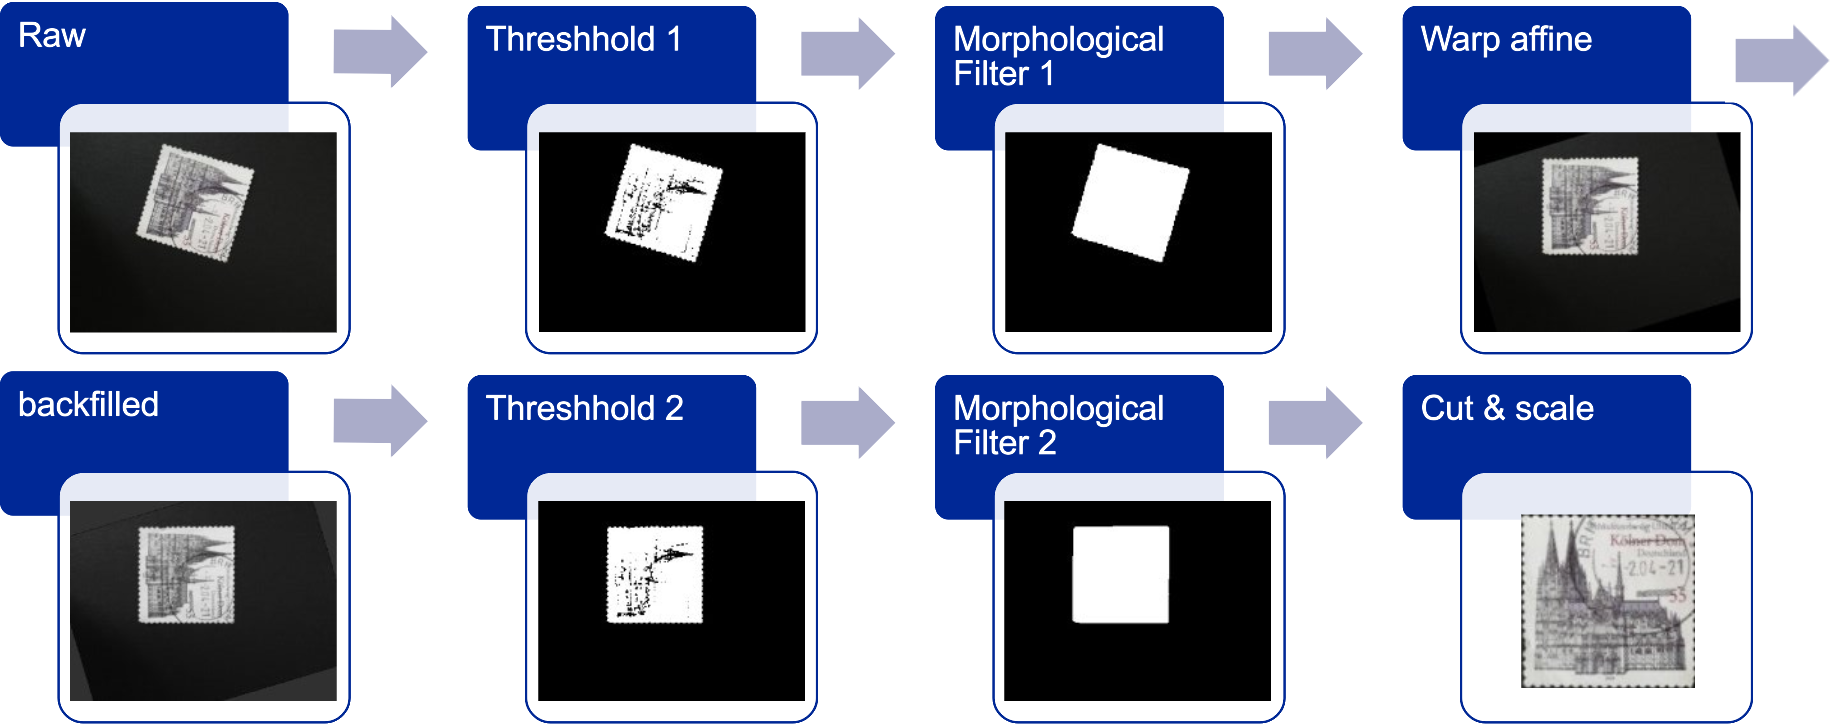
\includegraphics[width=\textwidth]{./bilder/bv_overview.png}
\caption{Übersicht über die Schritte der Bildvorverarbeitung}
\label{fig:bv_overview}
\end{figure}

\section{Beispiel ohne Komplikationen}
\label{sec_bv:paradebsp}

Im Folgenden wird der Ablauf der klassischen Bildverarbeitung an einem Beispiel, dass ohne weiteren Aufwand funktioniert, genauer erläutert.
\begin{figure}[!ht]

\begin{minipage}[t]{.75\linewidth}
Die beiden Bilder auf der rechten Seite sind Eingang und Ausgang des ersten Schrittes (Raw -> Threshold1). Das Raw Bild ist dabei ein RGB Bild, auf dem die Briefmarke in zufälliger Orientierung zu sehen ist. Der Hindergrund ist matt und schwarz-grau. Der Übergang zu Threshold1 wird mit einer Otsu Binarisierung bewerkstelligt. Es wird also in ein Graustufenbild übergegangen. Je nach Motiv der Briefmarke sind im Binärbild jedoch noch viele schwarze Stellen auf der Briefmarke. Dadurch resultiert die Marke nicht in einer einzelnen großen Kontur, sondern in vielen kleinen. Da wir jedoch erstmal das Bild gerade drehen wollen, bräuchten wir dafür eine einzige große, möglichst rechteckige, Kontur.
\end{minipage}
\hfill
\begin{minipage}[t]{.2\linewidth}
  \strut\vspace*{-\baselineskip}\newline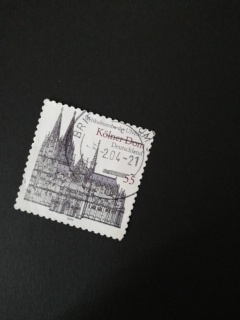
\includegraphics[width=\linewidth]{./bilder/start_dom}
  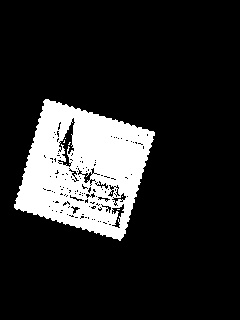
\includegraphics[width=\linewidth]{./bilder/bin1_dom}
  \caption{Übergang zu Threshold1}
  \label{fig:bv_th1}
\end{minipage}
\end{figure}
%%% ggf. weitere Abschnitte

\begin{figure}[h]
\begin{minipage}[t]{.75\linewidth}

Die Abbilung \ref{fig:bv_morph1} zeigt das Ergebnis des zweiten Schrittes des "klassischen" Teiles. Hier sind keine dunklen Stellen mehr auf der Fläche der Briefmarke. Das wurde durch die Verwendung eines morphologischen Filters zur Erweiterung und Schließung von Konturen erreicht. Es wurde dafür eine Quadratische Matrix mit Größe 11x11 verwendet. Bei einer Auflösung von 320x240 ist das ganz stattlich. 
\end{minipage}
\hfill
\begin{minipage}[t]{.2\linewidth}
\strut\vspace*{-\baselineskip}
\newline
  
\includegraphics[width=\linewidth]{./bilder/bin1morph}
  \caption{Übergang zu morph. Filter1}
  \label{fig:bv_morph1}
\end{minipage}
\end{figure}

\begin{figure}[h]
\begin{minipage}[t]{.75\linewidth}

Die Abbilung \ref{fig:bv_rotimg} zeigt, wie gut die Kontur aus dem Binärbild nun die Briefmarke repräsentiert. Der blaue Rahmen aus dem oberen Teil der rechten Abbildung wird mit der opencv Methode minAreaRect aus der Kontur des Binärbildes gewonnen. Mit dem Verdrehwinkel dieses Rechtecks kann nun das ursprüngliche Bild ausgerichtet werden. Dies geschieht mit Hilfe der warpAffine Funktion. Um diese zu nutzen muss vorher noch eine 2D Rotationsmatrix erstellt werden. Dafür werden wie Werte des Rechtecks verwendet. Das gerade gedrehte Bild ist im unteren Teil von Abbildung \ref{fig:bv_rotimg} zu erkenne.
\end{minipage}
\hfill
\begin{minipage}[t]{.2\linewidth}
  \strut\vspace*{-\baselineskip}\newline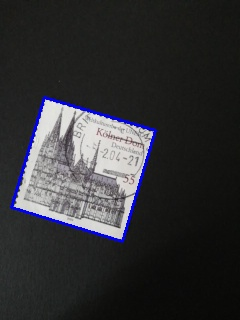
\includegraphics[width=\linewidth]{./bilder/minarearect_dom}
  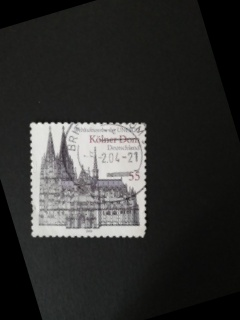
\includegraphics[width=\linewidth]{./bilder/rot_col}
  \caption{Rechteck, gerade gedrehtes Bild}
  \label{fig:bv_rotimg}
\end{minipage}
\end{figure}

\begin{figure}[h]
\begin{minipage}[t]{.75\linewidth}

Aus dem gerade gedrehten Bild der Abbildung \ref{fig:bv_rotimg} kann nun wieder ein Binärbild erstellt werden. Wenn man darauf wieder morphologische Filter anwendet, kann ein Binärbild wie in Abbildung \ref{fig:bv_morph2} erreicht werden. Das Rechteck aus dieser Kontur ist nun geeignet, um die Briefmarke aus dem gerade gedrehten Farbbild auszuschneiden. Das ausgeschnittene Bildstück hat natürlich von Marke zu Marke andere Größenverhältnisse. Die Briefmarken haben schließlich nicht nur unterschiedliche Formate, sondern sind auch nicht alle aus der perfekt gleichen Distanz fotografiert worden. Da das NN eine bestimmte Inputgröße erfordert, muss hier also noch was geändert werden.
\end{minipage}
\hfill
\begin{minipage}[t]{.2\linewidth}
\strut\vspace*{-\baselineskip}
\newline
  
\includegraphics[width=\linewidth]{./bilder/bin2morph}
  \caption{Übergang zu morph. Filter2}
  \label{fig:bv_morph2}
\end{minipage}
\end{figure}

\section{Mögliche Probleme}
\label{sec_bv:probleme}
In diesem Abschnitt sollen aufgetrettene Probleme geschildert und die gefundenen Lösungen gezeigt werden.\\

\begin{figure}[h]
\begin{minipage}[t]{.75\linewidth}

Wie in der Abbildung \ref{fig:bv_prob1} zu sehen ist, können gerade gedrehte Bilder nach der Binarisierung durch ein ungünstiges Motiv mehrere zureichend Große Konturen enthalten. Das Kriterium, das darüber entschieden hat, ob die Kontur eine potentielle Briefmarke ist, war vorher nur die Fläche. Demnach würden hier drei Bilder für das NN ausgeschnitten werden. Um das zu verhindern, wird hier auf eine Hierarchiebedingung zurück gegriffen. Diese lautet, dass nur Konturen ohne Parentkontur weiter genutzt werden. Im Beispiel rechts fallen deshalb die blau und die rot markierten Konturen weg und nur die richtige, grüne, bleibt übrig.
\end{minipage}
\hfill
\begin{minipage}[t]{.2\linewidth}
\strut\vspace*{-\baselineskip}
\newline
  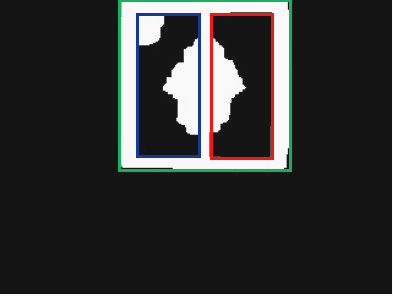
\includegraphics[width=\linewidth]{./bilder/prob1_bin}
  \caption{Binarisierung unzureichend}
  \label{fig:bv_prob1}
\end{minipage}
\end{figure}

\begin{figure}[h]
\begin{minipage}[t]{.75\linewidth}

Ein weiters Problem ist in Abbildung \ref{fig:bv_prob2} zu erkennen. Hier sind durch die Rotation große schwarze Flächen in den Ecken entstanden. Zur Binarisierung wird die Otsu Methode verwendet, der Schwellwert zur Binarisierung wird also automatisch und abhänig vom Bild und dessen Histogramm festgelegt. Normalerweise ist der Hintergrund dunkler als die Briefmarke. Durch die dunklen Ecken wird aber noch eine dritten, noch dunklere Fläche eingeführt. Dadurch verschiebt sich der Schwellwert in eine mittlere Helligkeitsstufe und Teile des Hintergrundes werden mit weiß binarisiert (oberer Teil der Abbildung). Um dieses Problem zu beheben wurden die die dunklen Stellen mit dem Mittelwert der Helligkeit des Orginalbildes nachgefärbt. Dadurch wird der Schwellwert deutlich schwächer beeinflusst und die Binarisieurng kann die Briefmarke wieder korrekt herausfiltern.
\end{minipage}
\hfill
\begin{minipage}[t]{.2\linewidth}
  \strut\vspace*{-\baselineskip}\newline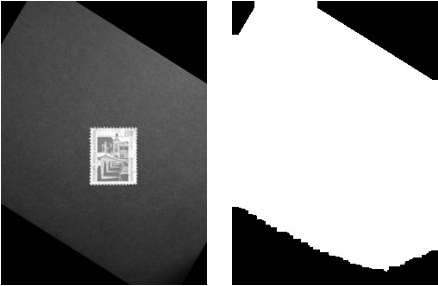
\includegraphics[width=\linewidth]{./bilder/prob2_bad_bin}
  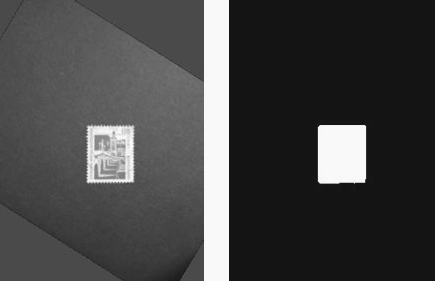
\includegraphics[width=\linewidth]{./bilder/prob2_good_bin}
  \caption{Darstellung des Binärisierungsproblems}
  \label{fig:bv_prob2}
\end{minipage}
\end{figure}


\begin{figure}[h]
\begin{minipage}[t]{.75\linewidth}

Das letzte Problem, das hier betrachtet werden soll, ist in Abbildung \ref{fig:bv_prob3} zu sehen. Auch wenn mit es mit dem menschlichen Auge schwer zu erkennen ist, ist das Bild sehr ungleichmäßig beleuchtet. Dadurch ist der ursprünglich schwarze Hintergrund in großen Bereichen sogar dunkler als die Briefmarke. Dadurch kann die Briefmarke gar nicht erst gerade gedreht werden. Im Verglich zum vorher gegangenen Problem entstehen die Kompliationen also nicht erst durch währen der Verarbeitung (wie zB. die schwarzen Ecken) sondern die Ursache dafür ist eine schlecht Qualität im Originalbild. Dieser Fall ist jedoch im ganzen Datensatz nur einmal aufgetretten. Da wir entschieden haben, dass dieser Verlust verkraftbar ist wurden hier keine weiteren Anstrengungen unternommen um das letzte Bild auch noch zu retten.´
\end{minipage}
\hfill
\begin{minipage}[t]{.2\linewidth}
  \strut\vspace*{-\baselineskip}\newline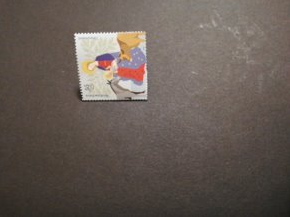
\includegraphics[width=\linewidth]{./bilder/prob3_pic}
  
\includegraphics[width=\linewidth]{./bilder/prob3_bad_bin}
  \caption{Darstellung des Binärisierungsproblems}
  \label{fig:bv_prob3}
\end{minipage}
\end{figure}

\section{Programmablaufplan}
\label{sec_bv:pap}
\begin{figure}[h]
\begin{minipage}[t]{.6\linewidth}

Die Abbildung \ref{fig:bv_pap} stellt eine Zusammenfassung des ganzen Kapitels \ref{sec:klass_bv} in Form eines Programmablaufplans dar. In der Abbildung wird zwar nur auf den Teil der gestempelten Bilder eingegangen, der  Teil der ungestempelten folgt jedoch dem gleichen Ablauf. Die Unterschiede sind, dass die Liste der Originalbildpfade anders ist und die als gut befundenen Bilder in ein anderes Verzeichnis gespeichert werden.\\
Der PAP zeigt, dass das Programm in zwei ineinander geschachtelten Schleifen abläuft. In der äußeren Schleife wird über die Liste der Bilder iteriert. Sollte eine Kontur mit ausreichender Größe durch die Binarisierung entstehen wird daraufhin in die zweite Schleif übergegangen. In dieser wird über die gefundenen Konturen nach der zweiten Binarisierng und Diletation iteriert. Zuerst wird dann die Fläche jeder Kontur abgefragt. Sollte die ausreichend sein ist die nächste Bedingung die Hierarchiebedingung, die das Problem aus \ref{fig:bv_prob1} löst. Wenn beide Bedingungen erfüllt wurden wird der Bildausschnitt dem Benutzer angezeigt. Sollte dieser den Ausschnitt für gut befinden kann er mit der "g" Taste der Tastatur die Briefmarke abspeichern. Mit der "b" Taste werden diverse Zwischenergebnisse in Form von Bilddateien in einen seperaten Ordner abgelegt. Dies erleichtert die Fehlersuche, ist aber für die Funktion des Programms unwichtig. Sollte das Bild weder gut noch ein interessanter Fehler sein kann mit einer beliebigen Taste mit dem nächsten Bild fortgefahren werden. Zusätzlich zur Anzeige der Bilder gibt eine Konsolenausgabe auch noch Aufschluss über die Anzahl der Schleifendurchläufe (Anzahl bearbeiteter Bilder und Konturen). Durch die beiden Schleifen und das zweimalige Binarisieren ist der Code zwar nicht besonders performant, aber gut nachvollziehbar. Da für jede Marke eine Benutzereingabe erforderlich ist, ist es egal das der Code nicht besonders effizient programmiert ist. Solange es dem Benutzer noch flüssig vorkommt wird praktisch keine Zeit verloren,  denn die Wartezeit auf die Eingabe macht die meiste Zeit aus.
\end{minipage}
\hfill
\begin{minipage}[t]{.35\linewidth}
\strut\vspace*{-\baselineskip}
\newline
  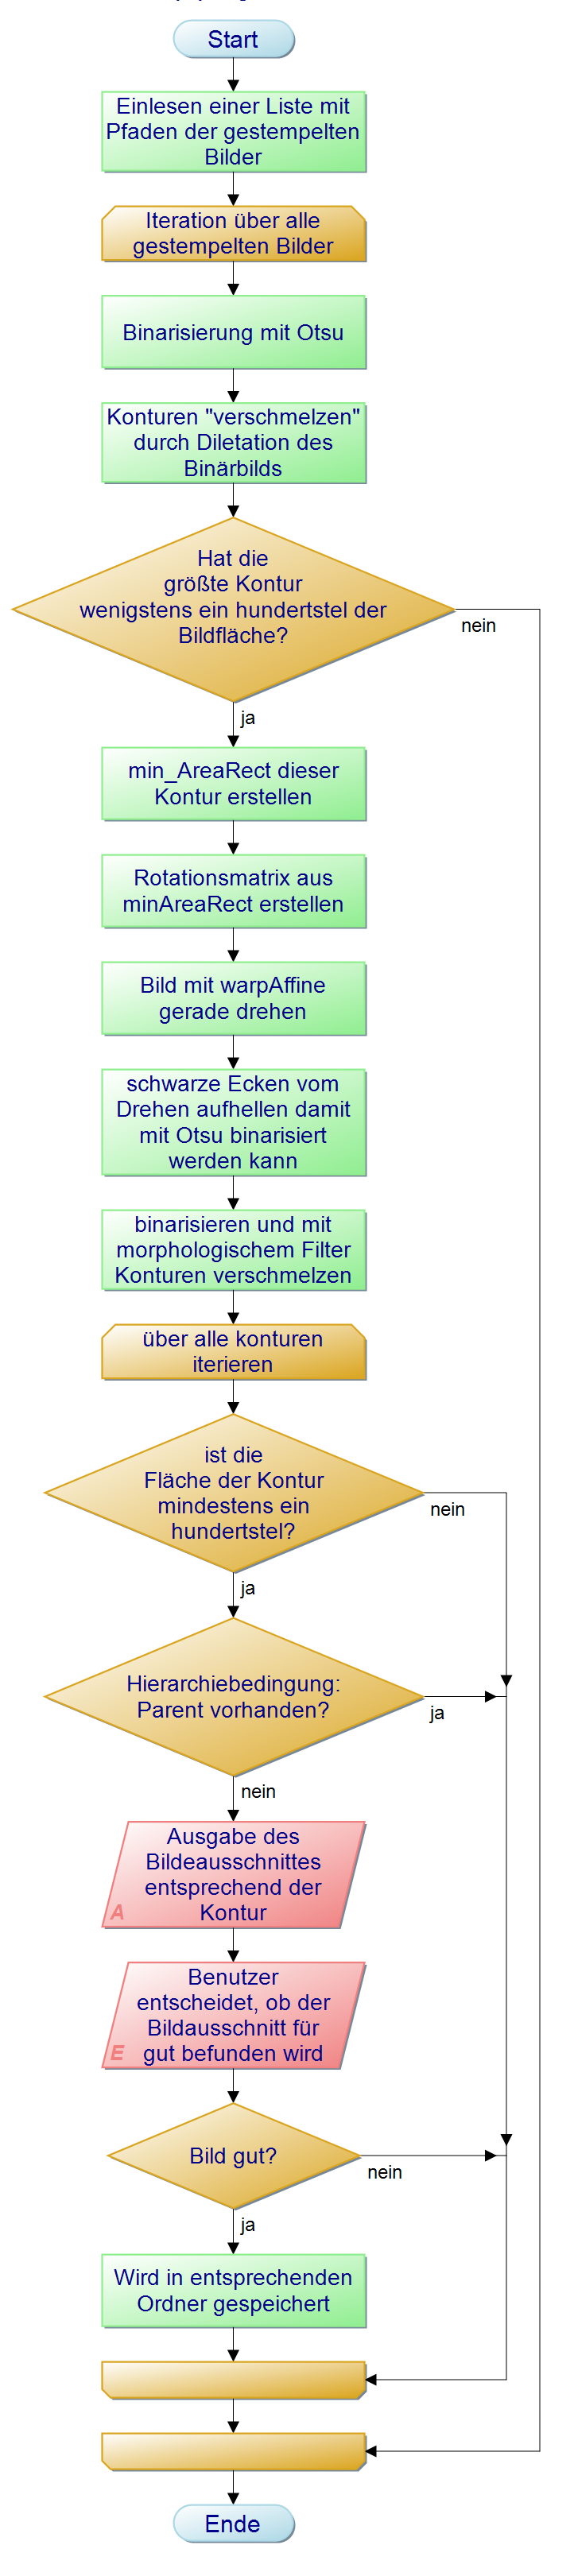
\includegraphics[width=\linewidth]{./bilder/BV_pap}
  \caption{Programmablaufplan}
  \label{fig:bv_pap}
\end{minipage}
\end{figure}

\chapter{Neuronales Netzwerk} % (fold)
\label{sec:nn}
Beim verwendeten NN handelt es sich um das MobileNetV2. Es kann für supervised learning Probleme zum Klassifizieren verwendet werden.

\section{Architektur und Vorgehen}
\label{sec_nn:architecture}


\section{Implementierung und Auswertung}
\label{sec_nn:impl}
\begin{figure}[h]
\begin{minipage}[t]{.71\linewidth}

Die Abbildung \ref{fig:nn_pap} zeigt, welche Schritte zur Implementierung in Pathon nötig waren. Zuerst ist natürlich wieder das Einlesen der Daten durchzuführen. Mit Hilfe einer assoziativen Liste (Dictionary) werden die Listen, die die Pfade zu den einzelnen Bildern enthalten, den beiden Klassen 0 und 1 zugewiesen. 0 steht in diesem Fall für gestempelt und 1 für ungestempelt. Als nächstes wird der Datensatz zufällig durchgemischt und dann in Verhältniss eins zu drei aufgeteilt. Der dreiviertelste Teil wird nachher zum Training verwendet. Mit dem kleineren Teil wird die Auswertung des Ergebnisses durchgeführt. Danach werden die Farbwerte aller Kanäle durch 255 geteilt, um den Wertebereich auf 0-1 zu reduzieren. Abschließend werden die Bilder des Datensatzes auf die Größe 224x224 geändert. Das NN kann schließlich nur mit Bildern gleicher Größe arbeiten. Damit ist die Arbeit am Datensatz abgeschlossen.
\end{minipage}
\hfill
\begin{minipage}[t]{.24\linewidth}
\strut\vspace*{-\baselineskip}
\newline
  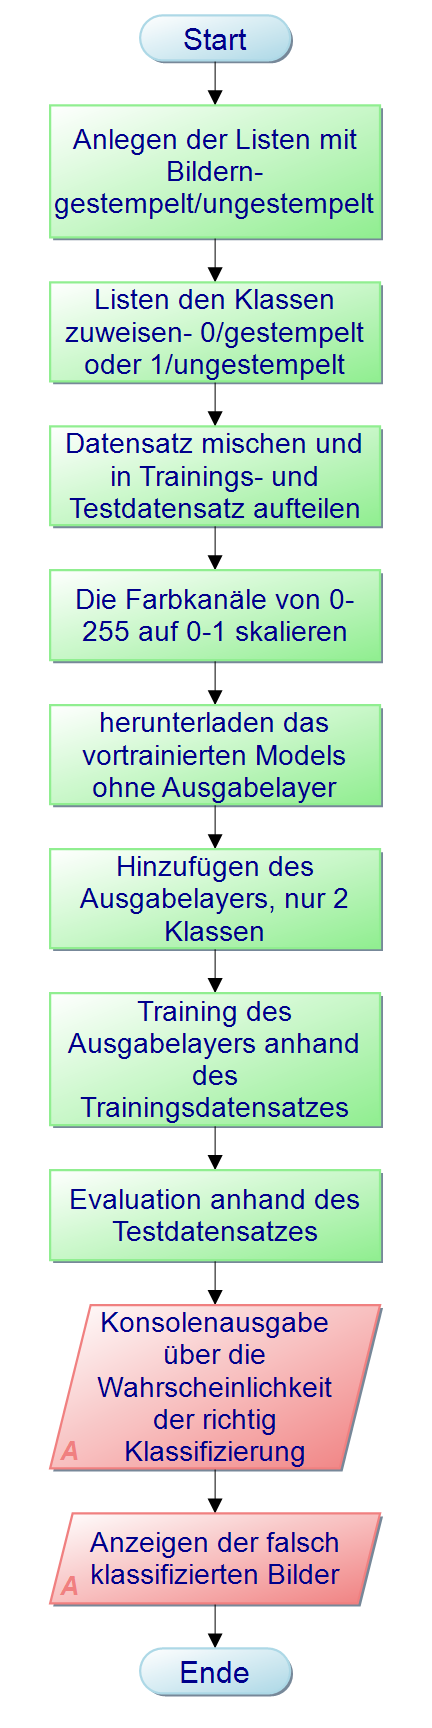
\includegraphics[width=\linewidth]{./bilder/Mobilenet}
  \caption{Programmablaufplan NN}
  \label{fig:nn_pap}
\end{minipage}
\end{figure}

\chapter{Fazit} % (fold)
\label{sec:fazit}

\ldots

% chapter fazit (end)

\appendix
\begin{thebibliography}{99}
\raggedright
%%% Printquellen zuerst
%%% Beispiel
\bibitem{Th11} Manuel René Theisen:
 \emph{Wissenschaftliches Arbeiten: Technik -- Methodik -- Form};
 15.~Auflage; Vahlen; München 2011;
 ISBN 978-3-8006-3830-7

%%% Internetquellen: Beispiel
\bibitem{hhneb} \emph{Hochschule Heilbronn};
 \url{http://www.hs-heilbronn.de/};
 abgerufen am 14.08.2010
\end{thebibliography}
\end{document}
